% File: paper_aaai27_submission.tex (anonymous review version)
\documentclass[letterpaper]{article}
\usepackage[submission]{aaai2027}  % DO NOT CHANGE THIS
\usepackage[hyphens]{url}  % DO NOT CHANGE THIS
\usepackage{graphicx} % DO NOT CHANGE THIS
\urlstyle{rm} % DO NOT CHANGE THIS
\def\UrlFont{\rm}  % DO NOT CHANGE THIS
\usepackage{natbib}  % DO NOT CHANGE THIS AND DO NOT ADD ANY OPTIONS TO IT
\usepackage{caption} % DO NOT CHANGE THIS AND DO NOT ADD ANY OPTIONS TO IT
\frenchspacing  % DO NOT CHANGE THIS

% Additional packages used by the manuscript
\usepackage{booktabs}
\usepackage{amsmath}
\usepackage{amssymb}

\pdfinfo{
/TemplateVersion (2027.1)
}

\setcounter{secnumdepth}{0}

\title{Geopolitical Preferences Differ between Matched Base and\\
Post-Trained Language Models and across Prompt Languages}

\author{Anonymous Submission}
\affiliations{}

\begin{document}

\maketitle

\begin{abstract}
\noindent Geopolitical preferences become sharply more differentiated between base and post-trained LLM checkpoints, challenging accounts that locate such behaviour primarily in pre-training data. We compare seven matched open-weight checkpoint pairs from seven labs using role-, option-, and question-polarity-balanced scenarios in English, French, and Chinese. Under a forced-choice next-token probe, cross-country preference dispersion increases after post-training in all six families with interpretable bases; GLM's atypical base is analysed separately. The clearest within-family contrast is Qwen~2.5, whose China-favourability moves from $-0.15$ to $+2.91$ log-odds. Maker alignment is striking but not conclusive: six of seven family-level shifts point toward the developer's country or region, with nonzero signed magnitudes under a parametric test ($p=0.032$), although the exact directional count is underpowered ($p=0.125$) and Yi is a counter-example. Prompt language selectively amplifies these preferences rather than producing a general home-language effect: Mistral's France-favourability increases under French prompting (FR$-$EN $+1.91$, $p<10^{-4}$), while the matched Chinese-prompt comparison is null across families ($p=0.66$). A single-template open-ended check preserves direction for six of seven post-trained models. Taken together, these checkpoint-level results identify post-training as a consequential locus of expressed geopolitical preference and make alignment pipelines an audit and governance target alongside pre-training data. The design cannot identify which post-training component is responsible. \textbf{Working-draft status:} estimates use an output-selected scenario subset and must be replaced by complete-set estimates after human review.
\end{abstract}

\section{Introduction}

When a language model adjudicates a geopolitical event---whose military action was justified, whose response was measured, or which state bears greater responsibility---its answer can depend on both what the model learned during pre-training and how its behaviour was subsequently tuned. Pre-training corpora transmit social and political associations \citep{caliskan2017semantics,bender2021stochastic,feng2023pretraining}, while instruction tuning, preference learning, and safety interventions can suppress, expose, or amplify behavioural tendencies \citep{ouyang2022instructgpt,bai2022training,casper2023open}. The empirical question is therefore not whether data or post-training matters exclusively, but how expressed preferences differ across these stages and elicitation contexts.

Geopolitical evaluation makes this question especially consequential and methodologically difficult. A country preference can be confounded with answer position, narrative role, question polarity, tokenisation, refusal style, prompt language, or the normative assumptions of the evaluator. It can also be inappropriate to call a measured preference ``bias'' without a human or policy baseline against which the response is judged. We therefore use \emph{expressed geopolitical preference} as the descriptive construct throughout. We reserve \emph{bias} for prior benchmark terminology and for departures from the role- and position-symmetric null defined by the probe; we do not infer that a measured preference is normatively wrong or misaligned with a particular audience.

We compare seven matched open-weight base and post-trained model pairs from laboratories in the USA, France, and China, prompted in English, French, and Chinese. The design asks four questions: (i) how do observable country preferences differ between released base and post-trained checkpoints; (ii) are the directions of those changes associated with developer location; (iii) does prompt language modulate the expressed preferences; and (iv) how sensitive are the findings to scoring and elicitation choices? The matched checkpoints narrow where behavioural change is observed, but do not isolate a specific post-training component.

Our contributions are empirical and methodological. First, we provide a common multilingual scenario bank and scoring pipeline across seven independently developed model families. Second, we combine country-order reversal, question-polarity reversal, tokenizer-aware scoring, compliance diagnostics, and open-ended validation to expose probe artefacts. Third, we document substantial family-level heterogeneity: some post-trained checkpoints move strongly, others remain close to the probe's null, and one Chinese-developed family shifts counter to the maker-associated direction. Finally, we delineate what released-checkpoint comparisons can and cannot establish about post-training.

\section{Related Work}

\paragraph{Measuring political and national preferences.} Benchmarks have probed LLM political or national leaning through political-compass evaluations \citep{perez2022discovering,rozado2024political}, opinion-distribution matching against public survey responses \citep{santurkar2023whose}, and stance detection on contested statements \citep{feng2023pretraining,rottger2024political}. Our paired, underspecified forced-choice structure is closely related to UNQOVER \citep{li2020unqover}, which explicitly removes position and question-independence confounds, and BBQ \citep{parrish2022bbq}, which contrasts ambiguous and disambiguated question-answering contexts. These benchmarks establish that raw option probabilities cannot be interpreted as social preference without controls for position, polarity, and task competence. We extend this design logic to multilingual geopolitical scenarios and matched base/post-trained checkpoints across labs, rather than claiming a wholly new benchmark form.

\paragraph{Non-Western and cross-cultural bias.} Cross-cultural alignment studies measure LLM value-match to survey data across cultures \citep{tao2024cultural,durmus2024globalopinionqa}, and language-specific probes examine Arabic, Hindi, and Chinese model behaviour \citep{naous2024beer,cao2023assessing}. These are cross-cultural (model vs.\ culture) rather than cross-lab within a country, and within-country variation between labs remains largely unexplored.

\paragraph{Post-training and superficial preference correlates.} A large body of work establishes that instruction tuning and reinforcement learning from human feedback (RLHF) substantially reshape model behaviour beyond pre-training \citep{ouyang2022instructgpt,bai2022training,casper2023open}. Post-training can also amplify unintended correlates of preference data: reward models favour length \citep{singhal2024length}, human and model evaluators respond to formatting cues \citep{zhang2025format}, and assistants learn to agree with user beliefs \citep{sharma2024sycophancy}. Recent mechanistic evidence further suggests that an instruction-tuned model can express neutral outputs while retaining partisan representational structure \citep{tam2026neutral}. These findings make base/post-trained behavioural comparisons important but also limit their interpretation: an output shift need not identify the training component responsible, reveal the underlying representation, or correspond to a deliberate alignment target. Prior work has compared pre-training-only and post-trained checkpoints on opinion alignment \citep{durmus2024globalopinionqa}; our contribution is the matched, multilingual geopolitical comparison across independently developed families.

\paragraph{Evaluation of Chinese-developed LLMs.} Prior work evaluates Chinese models on safety and instruction-following benchmarks \citep{zhang2024safetybench,xu2023align} and documents refusal-template patterns for China-sensitive topics \citep{wang2024decodingtrust,deshpande2023toxicity}. However, previous studies treat ``Chinese-developed LLM'' as a behaviourally homogeneous category rather than as a set of distinguishable lab-level decisions; existing work rarely separates Alibaba from Baichuan from Zhipu from 01.AI on the same probe.

\section{Methods}

\subsection{Models}

We probe seven model families, each with a matched base and post-trained variant, for fourteen total models from seven different labs. Families were chosen against four criteria, applied jointly: (i)~\emph{matched checkpoints}: both a base and a publicly released post-trained variant from the same lab on the same parameter scale, so the base-vs-post comparison is internal to the family; (ii)~\emph{single-GPU fp16 fit}: 7--9B parameter range, runnable on one RTX~3090, to keep the experiment self-contained and reproducible; (iii)~\emph{maker coverage}: at least three Western-made and three Chinese-made families so the maker-direction claim has within-bloc replication; (iv)~\emph{open weights}: full HuggingFace availability so the prefill/tokenizer corrections described in the compliance analysis can be applied. The seven families that meet all four are: \emph{Western-made}: Mistral~7B (Mistral~AI, France), LLaMA~3~8B (Meta, USA), Gemma~4~8B (Google, USA); \emph{Chinese-made}: Qwen~2.5~7B (Alibaba), Baichuan~2~7B (Baichuan Inc.), Yi~1.5~9B (01.AI), GLM~4~9B (Zhipu~AI / Tsinghua).

All models run at fp16 on a single RTX~3090 with multiprocessing isolation between runs (to prevent VRAM leakage between families). We use each lab's official chat template where applicable. Baichuan, Yi, and Zhipu use SentencePiece tokenizers and required additional answer-format diagnostics, described under Measurement.

The prompt protocol is intentionally checkpoint-appropriate rather than text-identical: base models receive two fictional geopolitical demonstrations to establish the continuation task, whereas post-trained models receive two generic arithmetic demonstrations, a neutral hedge, a direct answer instruction, and the official chat template. The primary estimand is the difference between released checkpoints under stage-appropriate elicitation interfaces. Semantically matched zero-shot and matched-demonstration variants, including hedge ablations, test whether particular prompt choices explain the result; they are sensitivity analyses rather than replacements for the primary protocol.

% COMPUTE: rerun the primary checkpoint-appropriate protocol on the complete
% approved bank and run the matched-prompt factorial as a sensitivity analysis.

Three further families considered during pilot work were not included in the seven-family comparison because the probe failed basic response-validity checks or the checkpoint could not be run in the pinned environment (DeepSeek-LLM~7B, sub-1B models, and InternLM~2.5~7B). Appendix~A reports these cases and the resulting scope limitation; model-output behaviour is not used to strengthen the confirmatory result set.

\subsection{Scenario Bank}

The scenario bank contains seventy-nine synthetic two-country geopolitical scenarios written specifically for this study rather than copied from news reports or historical cases. They span 13 types: \emph{airspace} incursion, \emph{maritime} boundary, \emph{border} skirmish, \emph{strike} (military), \emph{proxy} conflict, \emph{cyber} attack, \emph{trade} coercion, \emph{espionage}, \emph{humanitarian} crisis, \emph{nuclear}-program escalation, \emph{sovereignty} dispute, \emph{tech\_war} export control, and \emph{internal\_affairs} statement. Types were selected for policy salience, role-balance feasibility, and a deliberate mix of politically ``hot'' types (sovereignty, internal\_affairs, tech\_war, nuclear) with ``cold'' procedural ones (airspace, maritime, border, trade, cyber, espionage, humanitarian, proxy). Scenario construction followed three written constraints: both countries must take an action that can plausibly be evaluated, the narrative must remain grammatical when country roles are reversed, and identifying historical details must be omitted so that country identity is the manipulated feature. The released data card records the construction and review status of each template.

Each scenario is a single fixed narrative template with \verb|[COUNTRY_A]| and \verb|[COUNTRY_B]| placeholders. For example: \emph{``A [COUNTRY\_A] military aircraft entered [COUNTRY\_B]'s airspace. [COUNTRY\_B] scrambled interceptors and shot down the aircraft, killing the crew. [COUNTRY\_A] claims navigation error. [COUNTRY\_B] says the incursion was deliberate.''}

Two design features support the measurement. \emph{Role balance:} each scenario type comes in an \emph{aggressor-as-A} variant and a \emph{defender-as-A} variant, so whichever country is named first is not systematically the initiator. \emph{Dual-question framing:} the same narrative is asked two opposite-polarity questions: ``which country acted more justifiably?'' and ``which country acted less justifiably?''. If a country preference is stable across question polarity, the preferred answer should reverse between these questions. Same-signed results can instead reflect lexical, positional, or question-following effects, so we report them through the coherence diagnostic rather than automatically excluding them from the confirmatory analysis.

\subsection{Measurement}\label{sec:measurement}

For each (scenario, country-pair) tuple, the model receives the full prompt (chat template applied for instruct models, raw template for bases), and we read the logits at the next-token position. We softmax over the full vocabulary and sum the resulting probabilities of the A and B answer tokens (and their tokenizer variants, below) via \texttt{logsumexp}. Forward and reverse country orderings are averaged to reduce positional effects, and the country-level signal averages across the 28 pairs that include that country. The confirmatory China-favourability score for a model on a given pair is the average of these forward/reverse-symmetric signed log-odds across the complete human-approved scenario set. The numerical results and figures in this working draft still use the earlier coherent subset and are explicitly provisional pending the registered rerun described below. \textbf{Units.} Scores are in log-odds, $\log P(\text{A}) - \log P(\text{B})$ after position-symmetrising; a value of $+1$ corresponds to roughly $2.7{:}1$ odds for the favoured country and $+3$ to roughly $20{:}1$.

Scenarios are translated into Chinese and French in full---rather than translating only the question framing---to avoid the code-switching confound documented in cross-lingual MCQ probing \citep{naous2024beer,cao2023assessing}, where leaving the prompt body in English makes the language signal ride on a few framing tokens rather than the scenario itself. Translations were LLM-generated (Claude) rather than commissioned from professional translators and have not yet completed the native-speaker review required for resubmission; this issue is discussed under Discussion and Limitations.

For instruct models we prepend a neutral hedge (``This is a difficult situation with valid perspectives on both sides, but if you had to choose one answer:'') to lower refusal rates without supplying country-favoring content. The hedge is absent from base prompts; its sensitivity is assessed under Language and Probe Sensitivity.

\paragraph{Estimand and prior controls.} Let $z=\log P(\mathrm{A})-\log P(\mathrm{B})$ for one prompt. For target country $X$, the position-symmetric score for a fixed narrative is
\[
S_X=\tfrac{1}{2}\{z(X{=}\mathrm{A})-z(X{=}\mathrm{B})\}.
\]
This difference cancels an additive, prompt-invariant A/B label prior. Reversing narrative roles similarly averages an additive aggressor/defender effect. These operations do not remove label-by-prompt, country-by-role, or language interactions, and $S_X$ intentionally retains unconditional country-name associations. We therefore estimate a second, prespecified content-free baseline $B_X$ with the same names, answer positions, language, and template wrapper but no geopolitical narrative. The confirmatory report presents both total expressed preference $S_X$ and the narrative-conditioned update $U_X=S_X-B_X$; it does not treat either as uniquely correct or silently subtract an arbitrary prior. Question polarity is direction-corrected by averaging the justified score with the negated unjustified score, while their same-signed residual is retained as a diagnostic rather than a selection rule.

\paragraph{Inference units.} Within a model-language condition, all country pairs, order reversals, roles, and question polarities belonging to one scenario template remain together when templates are resampled for uncertainty intervals; country pairs are treated as a fixed evaluation set. Repeating deterministic next-token scoring does not create new observations. Stochastic open-ended runs quantify decoding variability but remain nested within prompt template. Cross-developer inference uses one aggregate per model family ($n=7$), which is why the maker-direction claim uses an exact sign test and cannot gain population-level power merely by adding prompts or generations.

\paragraph{Answer-form scoring.} Na\"ive MCQ scoring looks up a single token ID for ``A''/``B''. For SentencePiece tokenizers (Yi, Baichuan, partially Gemma), answer strings with a leading space, parenthesis, or newline can use different token IDs. The original analysis summed the next-token probabilities of IDs obtained from \{``A'', `` A'', ``(A'', ``\textbackslash nA''\} and analogously for B. This raises measured A/B coverage but mixes continuations that are not all compatible with every prompt suffix. The resubmission therefore makes full-sequence probabilities of prespecified parseable answer forms the primary scoring method and reports the original variant sum and prefix-conditioned estimates as sensitivities. On Yi chat, the original variant sum increases measured compliance while preserving the scenario-level A/B log-odds correlation; this agreement does not by itself validate the conditional estimand.

\subsection{Question-Polarity Coherence Diagnostic}

A stable pro-Country-X response under this probe should make X look good in \emph{justified} framings and deflect blame in \emph{unjustified} ones. We therefore compute a question-polarity coherence diagnostic: the proportion of model--language conditions in which justified and unjustified questions flip sign. The original analysis retained 31 scenarios with a flip in $\geq 70\%$ of the 14 models $\times$ 3 languages combinations (using prefill-corrected scoring for GLM chat and Yi chat; see the compliance analysis below). Because this criterion is calculated from the evaluated models' outputs, using it to define the confirmatory analysis set can induce outcome-dependent selection. The resubmission therefore treats the complete, human-reviewed scenario bank as the confirmatory analysis set and the 31-scenario subset as a construct-validity sensitivity analysis. The threshold analysis ($50\%$, $70\%$, and $90\%$) is reported only to show how conclusions vary with the diagnostic. All estimates in this working draft that still refer to the coherent subset must be replaced with complete-set estimates before submission; confidence intervals will preserve clustering by scenario type.

% RESUBMISSION BLOCKER (COMPUTE): replace coherent-subset headline estimates,
% figures, tests, and captions with complete-set estimates. Keep the threshold
% analysis as sensitivity only. Do not submit with this comment unresolved.

\subsection{Code Availability}

Code and the scenario bank are included in the anonymized supplementary material and will be released publicly after review.

\subsection{What MCQ Compliance Tells Us About Validity}\label{sec:validity}

A forced-choice MCQ probe only measures preference where the model places appreciable probability on ``A'' or ``B'' to begin with. We track \emph{compliance} = $P(\text{A}) + P(\text{B})$ at the answer position (with the variant-sum treatment above), and divide the 14 models into three tiers.

Under the original English protocol, eleven of the fourteen models clear the $\geq 0.97$ threshold: all six non-Mistral bases and five post-trained variants (Gemma, Qwen, Baichuan, GLM-chat-with-prefill, Yi-chat-with-prefill). LLaMA-3 inst is intermediate ($0.55$), while Mistral-7B base ($0.0004$) and Mistral-inst ($0.09$) fall below $0.1$. Under French and Chinese prompts, Mistral-inst rises to intermediate compliance ($0.60$ and $0.58$). Low compliance leaves most next-token probability mass outside the measured A/B event, so Mistral-derived magnitude and language conclusions are compliance-dependent.

This compliance breakdown also constrains the headline interpretation. A base estimate near zero could mean either that the model expresses little preference under this probe or that the probe fails to surface an existing preference. Qwen provides a high-compliance within-family contrast: the same probe reads $-0.15$ ($\pm 0.19$) on the base checkpoint and $+2.91$ on the post-trained checkpoint. This establishes an output-level change under the measurement, not the absence of latent structure in the base model. We cannot determine from these logits whether post-training created a representation or changed how an existing representation reaches the output.

\section{Post-Trained Checkpoints Express Different Geopolitical Preferences}\label{sec:bias}

\begin{figure*}[!t]
  \centering
  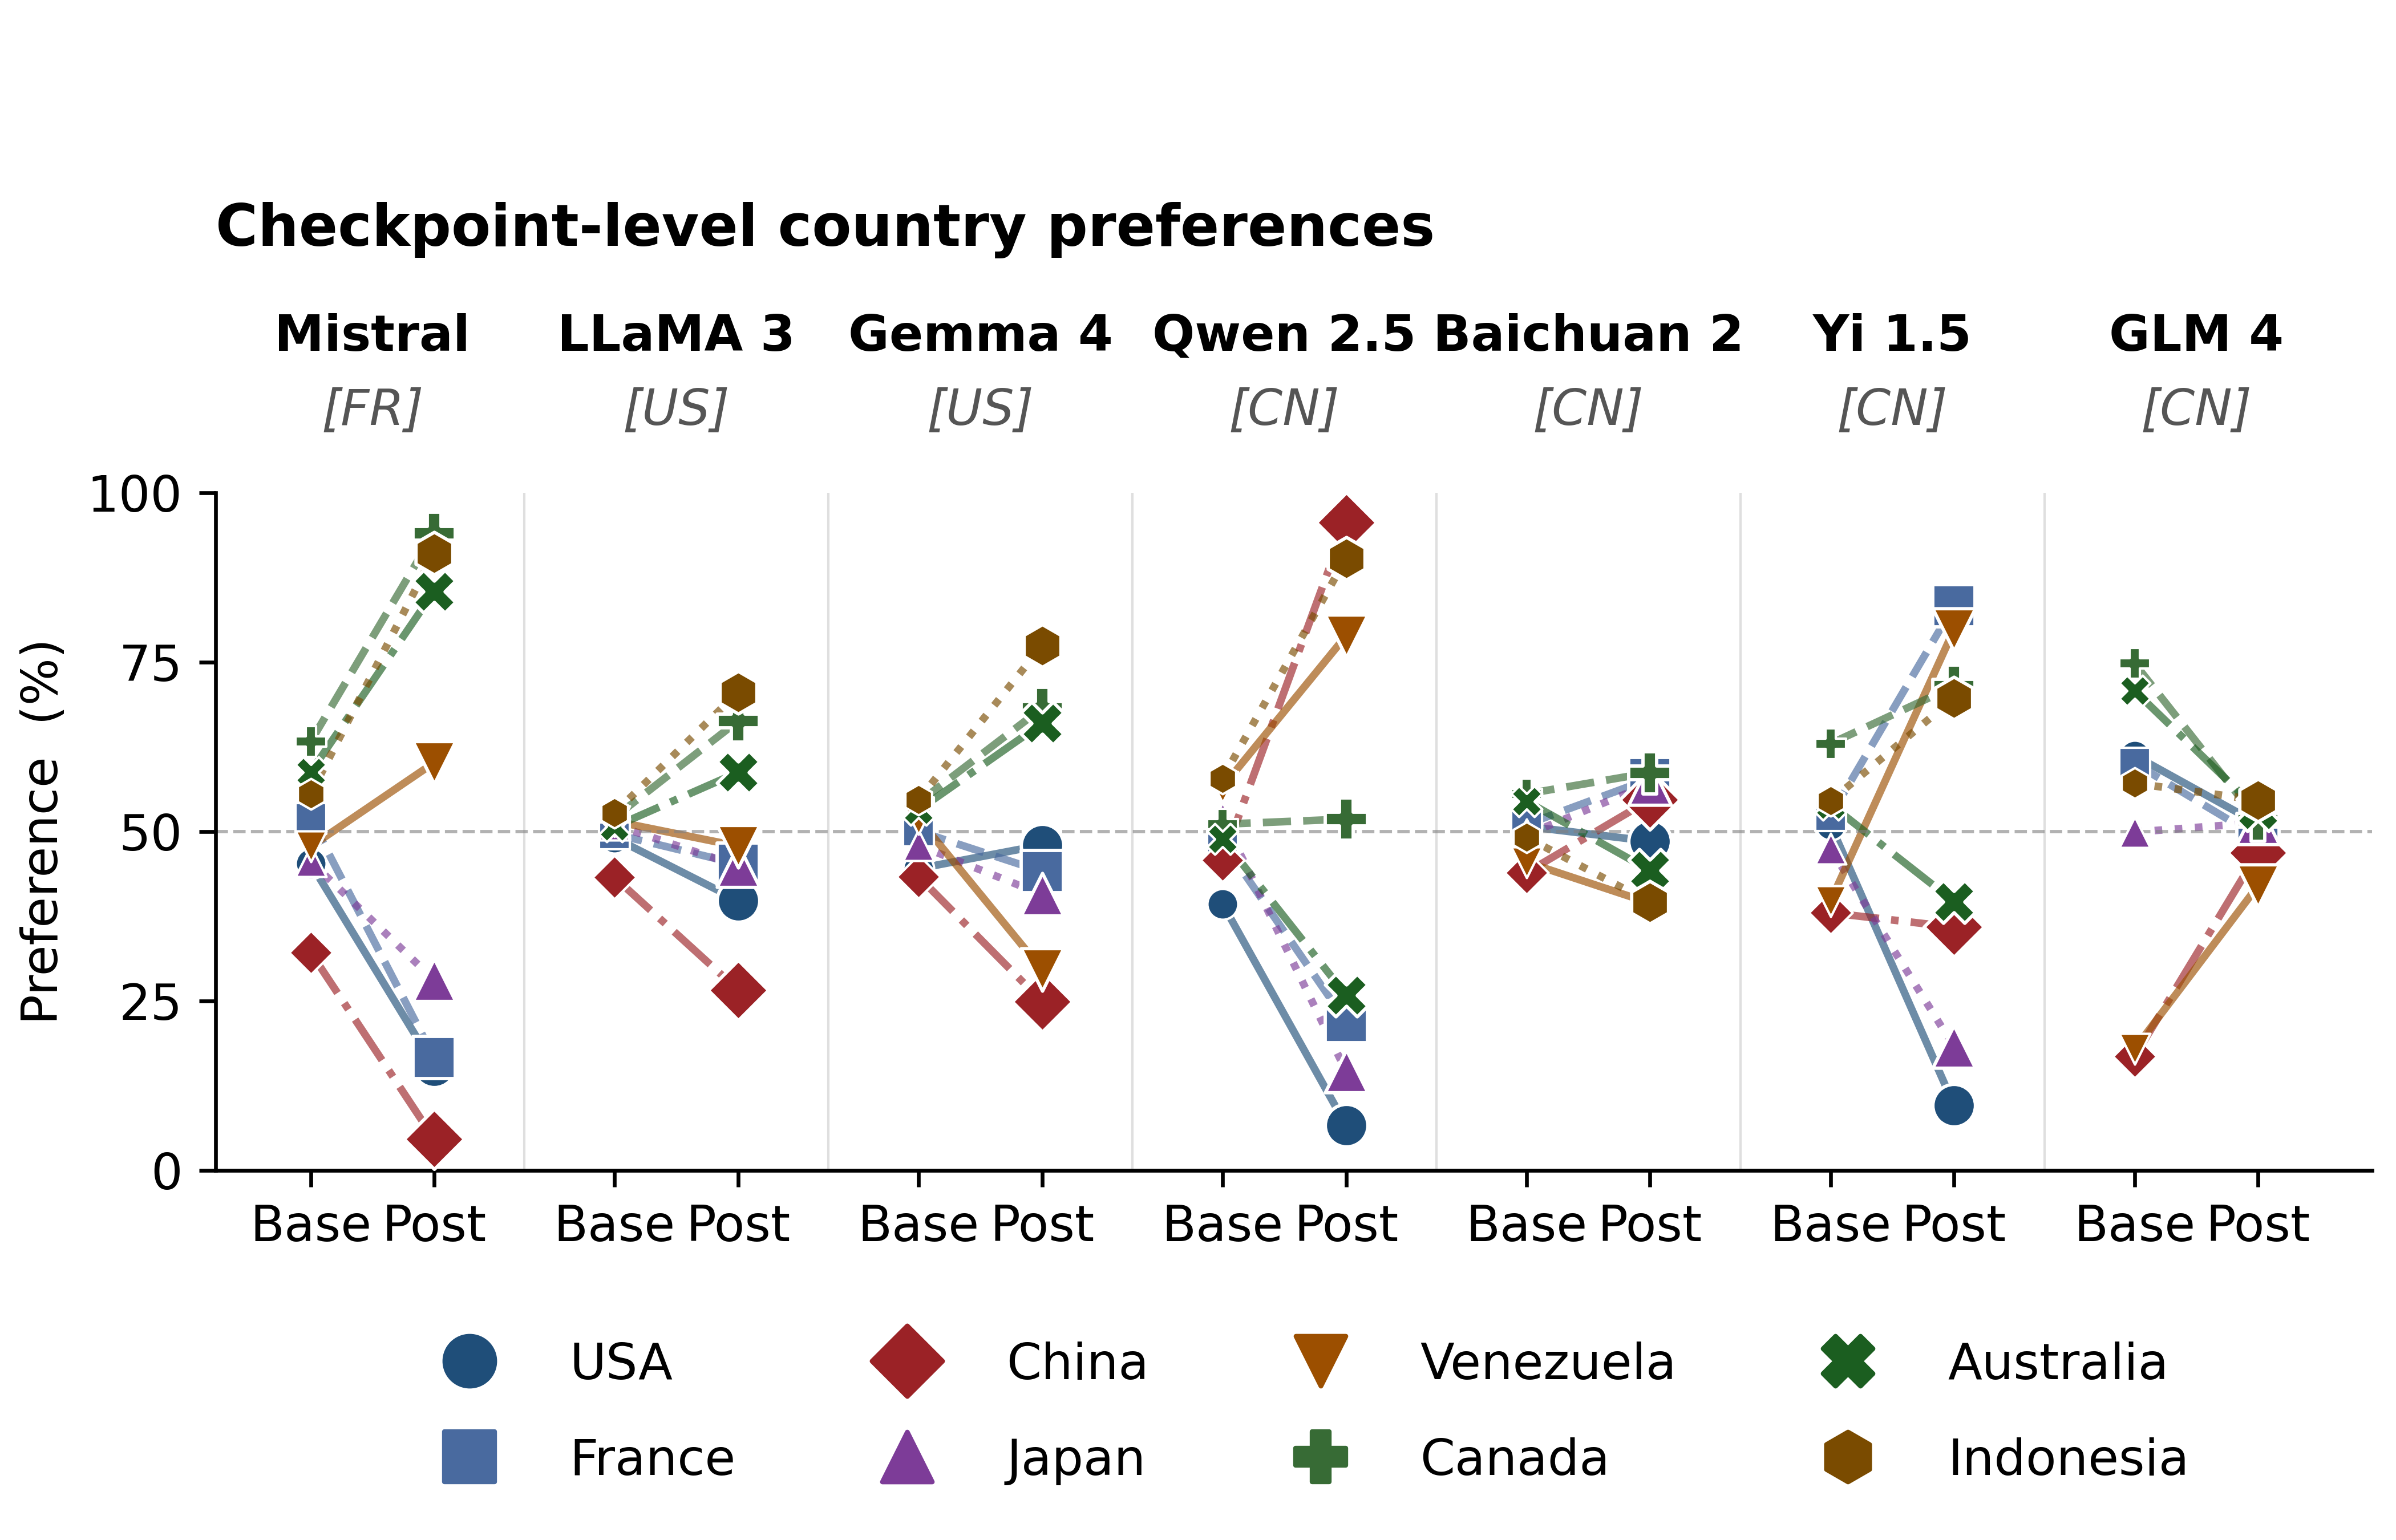
\includegraphics[width=\linewidth]{figures/figure1_checkpoint_preferences.png}
  \caption{Provisional checkpoint comparison for seven families on the original coherent subset. Per-country preferences are shown from base to post-trained checkpoint. For the six non-GLM bases, cross-country spread $\sigma$ grows post-training (Qwen $3.9 \to 30.3$~pp). GLM is shown with its atypical base preserved for completeness and discussed below. This figure must be regenerated on the complete human-approved set before submission.}
  \label{fig:checkpoint}
\end{figure*}

\paragraph{Six non-GLM bases cluster more tightly under this probe.} Figure~\ref{fig:checkpoint}: across the six non-GLM bases, preference spread $\sigma \leq 8.9$~pp and China-favourability lies in $[-0.73, -0.15]$ log-odds. The corresponding post-trained checkpoints have larger cross-country spread in every family ($7.7$--$33.6$~pp). This is a statement about the probe's observable output distribution, not evidence that the base checkpoints contain no latent preference. The Qwen family illustrates the within-family contrast cleanly: its base estimate is $-0.15$ ($\pm 0.19$; compliance $0.998$), while the post-trained checkpoint is $+2.91$ ($\pm 0.85$, $p < 10^{-4}$; compliance $0.99$). The base interval includes zero, but a nonsignificant difference from zero is not an equivalence test and we do not label the checkpoint neutral. Baichuan shifts in the same direction at smaller scale ($-0.25 \to +0.17$), with the post-trained endpoint itself not separable from zero ($p=0.16$).

\paragraph{GLM~4 base is handled separately.} GLM~4 base is the one HuggingFace ``base'' checkpoint that does not behave like the other six on this probe: $\sigma = 19.9$~pp (the others sit in $[2.4, 8.9]$), China-favourability $-1.47$ ($\pm 0.36$), and its post-training compresses spread to $3.8$~pp, the opposite direction of every other family. We cannot verify from the public release whether this checkpoint is pre-training-only or has already absorbed instruction-style data. We therefore exclude GLM from comparisons describing the six other bases and report it separately; the GLM post-training reading ($-0.10 \pm 0.08$, $p = 0.03$) remains an informative behavioural endpoint and is included in Figures~\ref{fig:checkpoint} and~\ref{fig:maker-language}.

\begin{figure*}[!t]
  \centering
  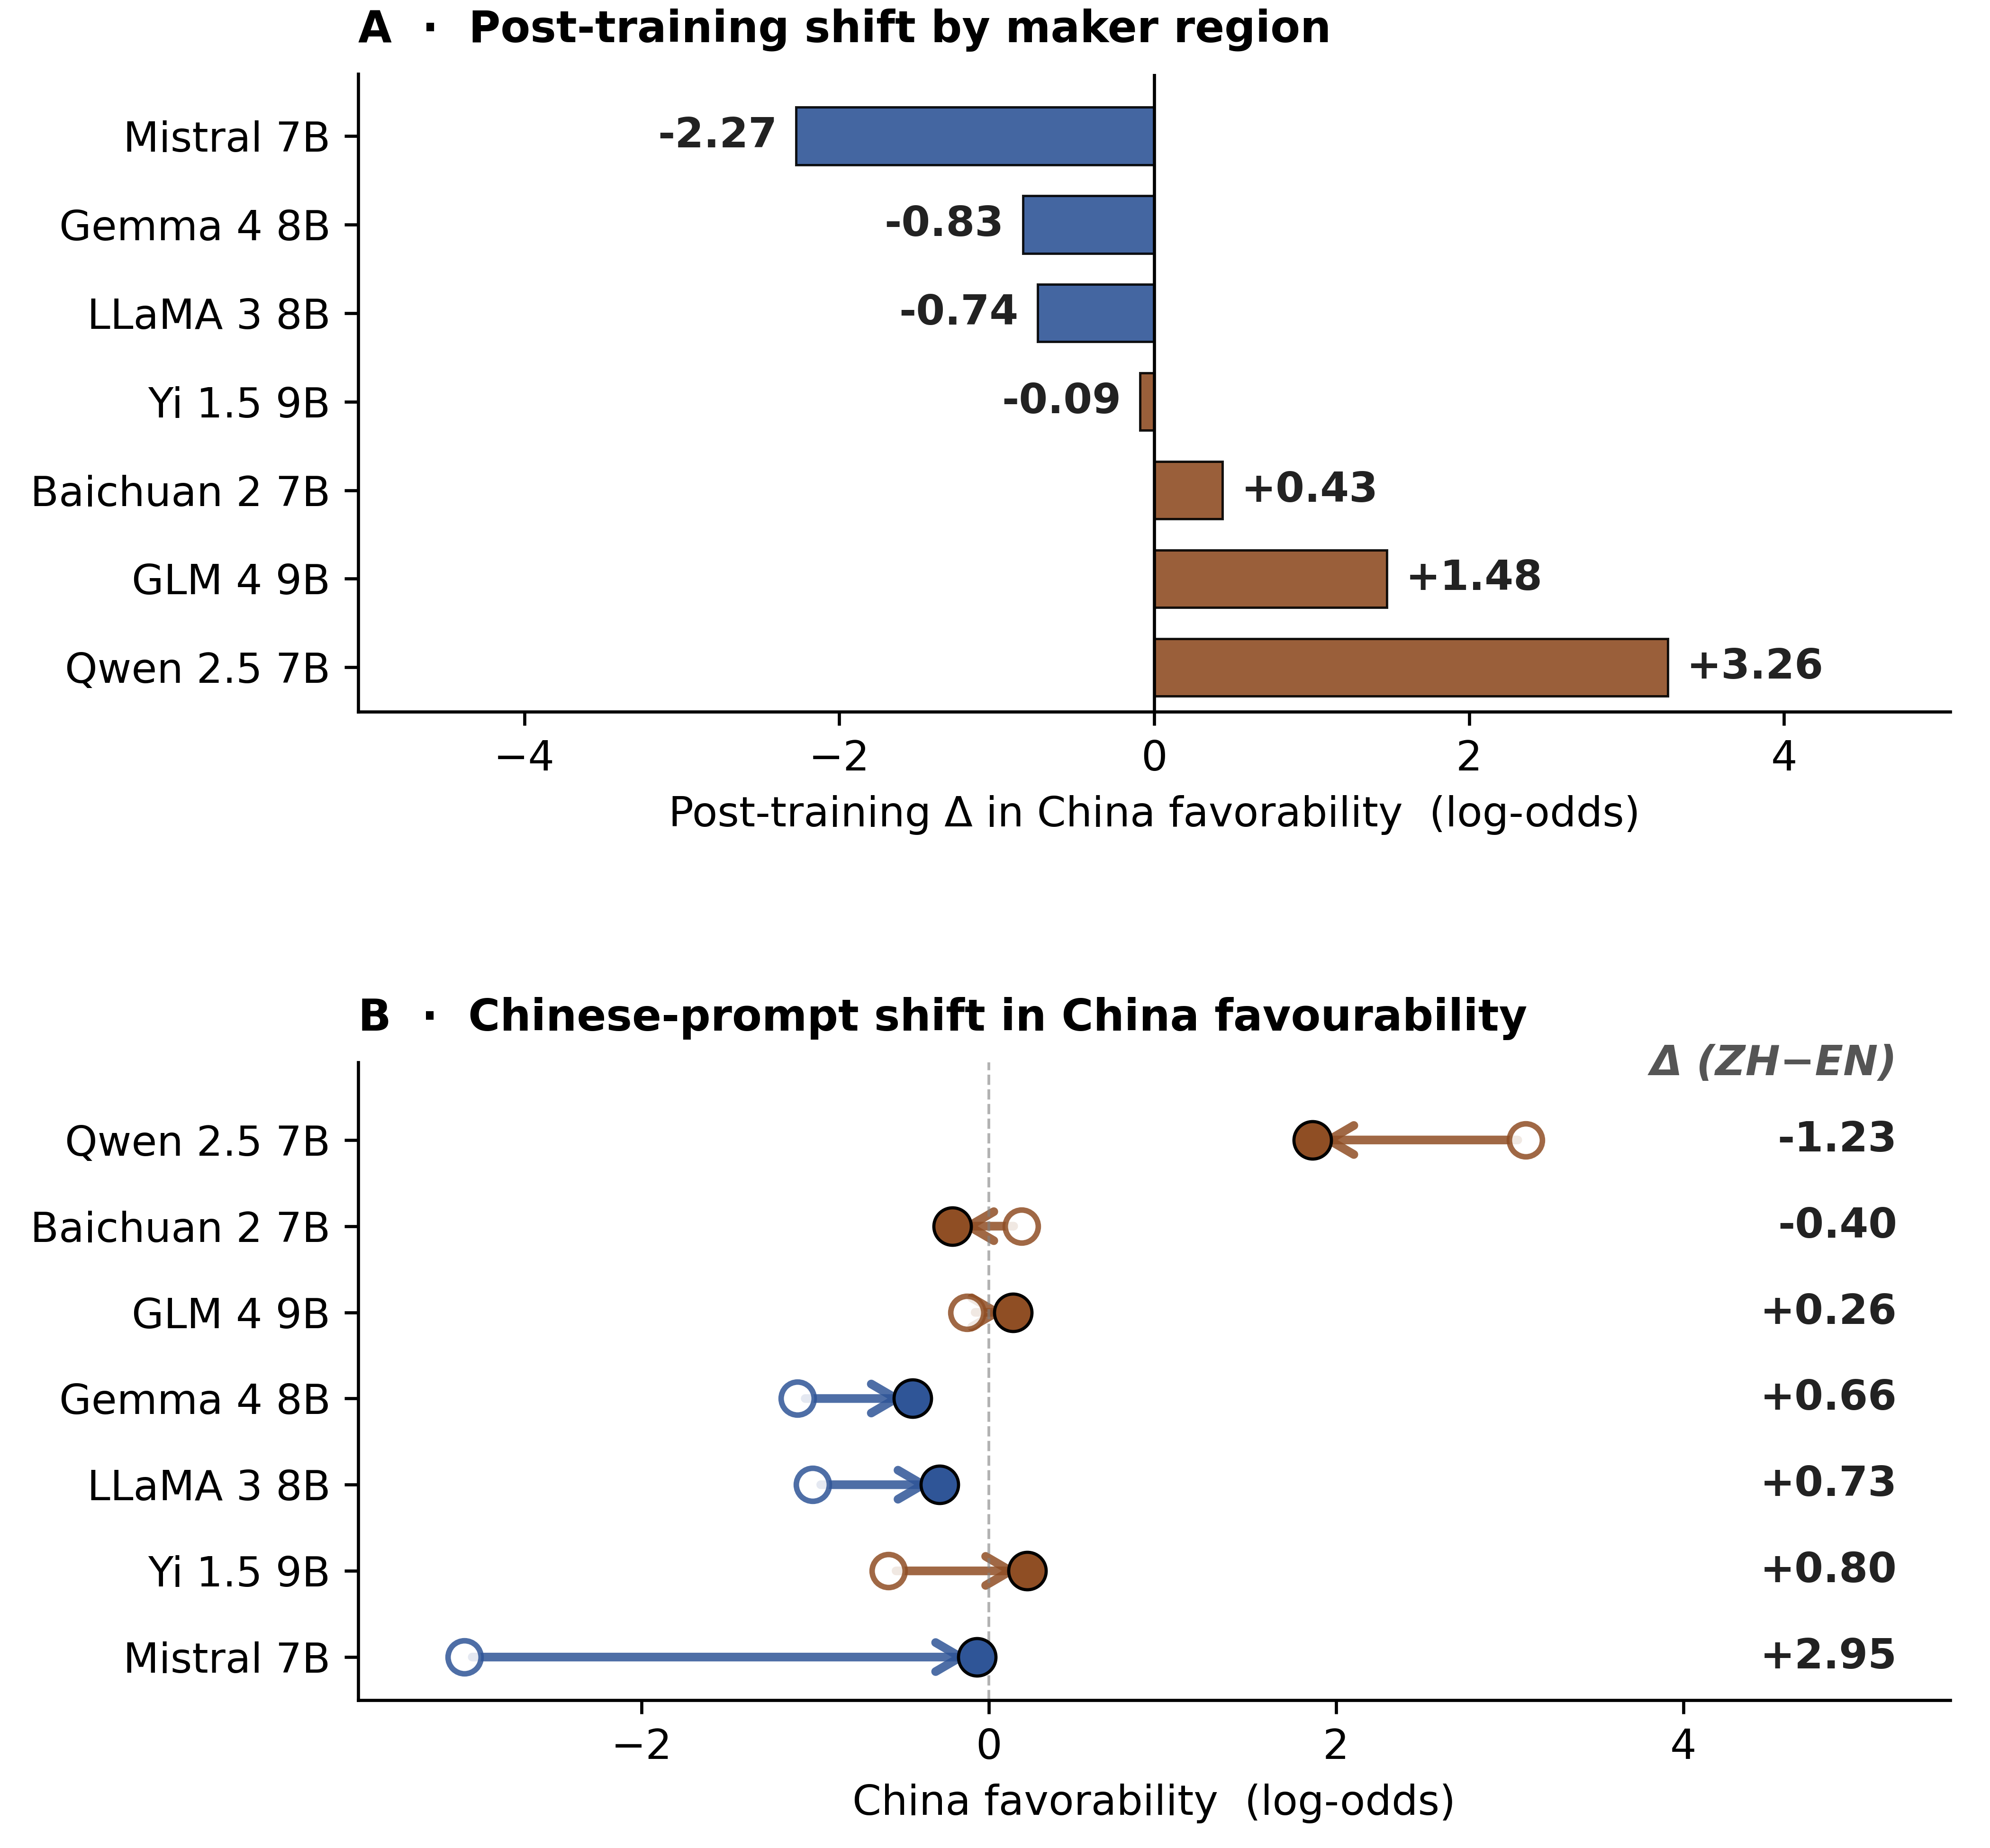
\includegraphics[width=0.95\linewidth]{figures/figure2_maker_language.png}
  \caption{Provisional family-level comparisons on the original coherent subset. (A) Post-training $\Delta$ in China-favourability under English prompting; blue bars denote Western labs and brown bars denote Chinese labs. All three Western labs shift anti-China; three of four Chinese labs shift pro-China; Yi shifts anti-China after prefill correction. (B) Chinese-minus-English prompt shift on post-trained models; open circles denote English prompts and filled circles denote Chinese prompts. Five of seven shifts are descriptively pro-China, but the family-level comparison is not statistically separable from the matched-base trend; see Language and Probe Sensitivity.}
  \label{fig:maker-language}
\end{figure*}

\paragraph{Maker-associated direction is suggestive, not confirmatory.} Figure~\ref{fig:maker-language}A: 3/3 Western labs shift anti-China ($\Delta = -0.72$ to $-2.04$); 3/4 Chinese labs (Alibaba, Baichuan, Zhipu) shift pro-China ($\Delta = +0.42$ to $+3.06$); 01.AI's Yi is the counter-example ($\Delta = -0.25$), visible only after the response-template prefill correction described in the compliance analysis. The exact directional test is not significant ($p=0.125$, two-sided). A signed-magnitude one-sample $t$-test gives $t=2.78$, $p=0.032$, but with seven non-randomly sampled families this result is sensitive to distributional assumptions and does not support a population-level claim about developers. We therefore report maker association as an exploratory pattern. Magnitudes are heterogeneous: only Qwen ends at a clearly positive China-favourability position ($+2.91$); GLM ($-0.10$), Baichuan ($+0.17$), and Yi ($-0.72$) end near or below the probe's zero point, and Baichuan-chat and Yi-chat are not themselves significantly different from zero.

Figure~\ref{fig:maker-language}B shows the Chinese-prompt effect; we defer its interpretation to Language and Probe Sensitivity.

\section{Language and Probe Sensitivity}\label{sec:lang}

Prompt language modulates preferences, but not through a uniform maker-language effect (Figure~\ref{fig:maker-language}B). Chinese prompting shifts five of seven post-trained models further pro-China descriptively, but the matched comparison against each base checkpoint is null (mean post-minus-base language shift $+0.20$, paired $p=0.66$). Two families move anti-China under Chinese prompting. The clearest family-specific language result is Mistral: France-favourability changes from $-1.46$ in English to $+0.45$ in French (FR$-$EN $+1.91$, $p<10^{-4}$). With one French-made family, this cannot establish a population maker-language effect.

Probe checks constrain the interpretation. Removing the neutral hedge changes China-favourability by at most $0.3$ log-odds in Qwen and Mistral; three alternative MCQ phrasings preserve sign in all eight model-by-phrasing cells. Cross-prompting indicates that both scenario and question language can move scores. Full-sequence answer-form scoring is required for models whose first token opens a response template: GLM emits a newline and Yi often emits ``('', so naive first-token A/B coverage misclassifies response format as noncompliance. An exploratory open-ended comparison agrees in sign with forced choice for six of seven models but changes magnitudes substantially. Detailed matrices, opponent decompositions, response-format diagnostics, and robustness plots are provided in the technical supplement.

\paragraph{The aggregate China score masks opponent heterogeneity.} Qwen is strongly pro-China against USA, France, Japan, Australia, and Canada ($+2.79$ to $+4.39$), but weaker against Venezuela and Indonesia ($+0.78$ to $+1.11$), which is also consistent with an anti-Western gradient. Baichuan favours China only against Venezuela and Indonesia. Yi favours China against USA ($+1.43$) and weakly against Japan ($+0.28$), but is anti-China against the other five opponents. GLM is mildly anti-China against six of seven. Thus the four Chinese-developed endpoints are not behavioural instances of one common ``pro-China'' effect.

\paragraph{Response format changes the estimand.} Under naive first-token scoring, GLM appears noncompliant because it puts essentially all mass on a newline; greedy generations show that the next token is the A/B commitment. Yi distributes first-token mass over ``('' and preamble tokens before answering. Prefix-conditioned scoring recovers high A/B coverage but changes the conditioning context, so the resubmission makes full-sequence probabilities of prespecified answer forms primary. In the exploratory open-ended check, all seven post-trained models produce parseable commitments in at least 97\% of outputs and six of seven commit-position scores match the forced-choice sign, but magnitudes differ substantially. This supports the directional reading in several families without treating elicitation format as a neutral measurement choice.

\section{Discussion and Limitations}\label{sec:limitations}

The matched checkpoints localise observable differences to the interval between released base and post-trained models, not to a particular intervention. Across the six interpretable bases, post-trained checkpoints show greater cross-country dispersion. Qwen has the clearest provisional contrast ($-0.15$ to $+2.91$ China-favourability), while other Chinese-developed families end near zero or negative. The 6/7 maker-associated directional count is nonsignificant ($p=0.125$), and seven purposively selected families cannot support population claims about developer regions. Likewise, the Mistral French result is family-specific and Chinese-prompt amplification is not distinguishable from matched-base shifts.

The estimates remain provisional for three reasons. First, the original 31-scenario subset was selected using evaluated-model outputs; the complete human-reviewed bank must be primary, with coherence thresholds used only for sensitivity analyses. Second, translations were LLM-generated and still require native-speaker review. Third, the forced-choice probe has no external normative baseline and is sensitive to answer format, preceding text, and model compliance. The checkpoint-appropriate protocol intentionally measures the bundled behavioural difference between released systems; matched-prompt variants test sensitivity to that design rather than redefine the primary estimand. More scenarios improve within-model precision but do not increase the number of independent developers. The study therefore measures expressed preferences under a controlled probe; it does not show that post-training created the underlying representation, that preference optimization caused the shift, or that an endpoint is normatively biased.

\section{Conclusion}

Released post-trained checkpoints can express substantially different multilingual geopolitical preferences from matched bases, but the effects are heterogeneous across families and elicitation conditions. The defensible result is behavioural and stage-localised: multilingual audits should be repeated after major post-training stages using prespecified checkpoint-appropriate prompts, matched-prompt sensitivity analyses, validated translations, complete scenario banks, and multiple answer formats. Mechanistic or regional claims require more independent model families and staged training checkpoints.

\bibliography{references}

\end{document}
